
%	PACKAGES AND OTHER DOCUMENT CONFIGURATIONS
%----------------------------------------------------------------------------------------

\documentclass[
12pt, % The default document font size, options: 10pt, 11pt, 12pt
%oneside, % Two side (alternating margins) for binding by default, uncomment to switch to one side
english, % ngerman for German
doublespacing, % Single line spacing, alternatives: onehalfspacing or doublespacing
%draft, % Uncomment to enable draft mode (no pictures, no links, overfull hboxes indicated)
nolistspacing, % If the document is onehalfspacing or doublespacing, uncomment this to set spacing in lists to single
liststotoc, % Uncomment to add the list of figures/tables/etc to the table of contents
%toctotoc, % Uncomment to add the main table of contents to the table of contents
parskip, % Uncomment to add space between paragraphs
%nohyperref, % Uncomment to not load the hyperref package
headsepline, % Uncomment to get a line under the header
%chapterinoneline, % Uncomment to place the chapter title next to the number on one line
%consistentlayout, % Uncomment to change the layout of the declaration, abstract and acknowledgements pages to match the default layout
twoside
]{MastersDoctoralThesis} % The class file specifying the document structure

\usepackage[utf8]{inputenc} % Required for inputting international characters
\usepackage[T1]{fontenc} % Output font encoding for international characters
\usepackage{wrapfig}

\usepackage{mathpazo} % Use the Palatino font by default

\usepackage[backend=bibtex,style=authoryear,natbib=true]{biblatex} % Use the bibtex backend with the authoryear citation style (which resembles APA)

\addbibresource{example.bib} % The filename of the bibliography

\usepackage[autostyle=true]{csquotes} % Required to generate language-dependent quotes in the bibliography

\usepackage{pgfplots}
    \pgfplotsset{compat=1.12,}
\usepackage{amsmath,amsfonts,amsthm,amssymb,graphicx,mathtools,tikz,hyperref} \renewcommand\qedsymbol{$\blacksquare$}
\usetikzlibrary{positioning}
\newcommand{\N}{\mathbb{N}}
\newcommand{\Z}{\mathbb{Z}}
\newcommand{\Q}{\mathbb{Q}}
\newcommand{\CX}{\mathbb{C}}
\newcommand{\R}{\mathbb{R}}
\newcommand{\F}{\mathbb{F}}
\newcommand{\ita}[1]{\textit{#1}}
\newcommand{\com}[2]{#1\backslash#2}
\newcommand{\oneton}{\{1,2,3,...,n\}}
\newcommand\idea[1]{\begin{gather*}#1\end{gather*}}
\newcommand\ef{\ita{f} }
\newcommand\eff{\ita{f}}
\newcommand\proofs[1]{\begin{proof}#1\end{proof}}
\newcommand\inv[1]{#1^{-1}}
\newcommand\setb[1]{\{#1\}}
\newcommand\en{\ita{n }}
\newcommand{\vbrack}[1]{\langle #1\rangle}

\theoremstyle{plain}
\newtheorem{theorem}{Theorem}[section]
\newtheorem{lemma}[theorem]{Lemma}
\newtheorem{proposition}[theorem]{Proposition}
\newtheorem*{corollary}{Corollary}

\theoremstyle{definition}
\newtheorem*{definition}{Definition}
\newtheorem{conjecture}{Conjecture}
\newtheorem{example}{Example}

\theoremstyle{remark}
\newtheorem*{remark}{Remark}
\newtheorem*{claim}{Claim}
\newtheorem*{note}{Note}



%----------------------------------------------------------------------------------------
%	MARGIN SETTINGS
%----------------------------------------------------------------------------------------

\geometry{
	paper=letterpaper, % Change to letterpaper for US letter
	inner=2.5cm, % Inner margin
	outer=3.8cm, % Outer margin
	bindingoffset=.5cm, % Binding offset
	top=1.5cm, % Top margin
	bottom=1.5cm, % Bottom margin
	%showframe, % Uncomment to show how the type block is set on the page
}

%----------------------------------------------------------------------------------------
%	THESIS INFORMATION
%----------------------------------------------------------------------------------------

\thesistitle{Elliptic Curve Cryptosystems} % Your thesis title, this is used in the title and abstract, print it elsewhere with \ttitle
\supervisor{Prof. Janwa } % Your supervisor's name, this is used in the title page, print it elsewhere with \supname
\author{Ray Rosario, Alec Zabel-Mena} % Your name, this is used in the title page and abstract, print it elsewhere with \authorname

\subject{Abstract Algebra} % Your subject area, this is not currently used anywhere in the template, print it elsewhere with \subjectname
\keywords{Elliptic Curve, Cryptography, Massey-Omura cryptosystem} % Keywords for your thesis, this is not currently used anywhere in the template, print it elsewhere with \keywordnames
\university{\href{http://www.university.com}{University of Puerto Rico}} % Your university's name and URL, this is used in the title page and abstract, print it elsewhere with \univname
\department{\href{http://department.university.com}{Department of Mathematics}} % Your department's name and URL, this is used in the title page and abstract, print it elsewhere with \deptname



\begin{document}

\frontmatter % Use roman page numbering style (i, ii, iii, iv...) for the pre-content pages

\pagestyle{plain} % Default to the plain heading style until the thesis style is called for the body content

%----------------------------------------------------------------------------------------
%	TITLE PAGE
%----------------------------------------------------------------------------------------

\begin{titlepage}
\begin{center}

\vspace*{.06\textheight}
{\scshape\LARGE \univname\par}\vspace{1.5cm} % University name
\textsc{\Large Research Project}\\[0.5cm] % Thesis type
\subjectname

\HRule \\[0.4cm] % Horizontal line
{\huge \bfseries \ttitle\par}\vspace{0.4cm} % Thesis title
\HRule \\[1.5cm] % Horizontal line
 
\begin{minipage}[t]{0.4\textwidth}
\begin{flushleft} \large
\emph{Author:}\\
{\authorname} % Author name - remove the \href bracket to remove the link
\end{flushleft}
\end{minipage}
\begin{minipage}[t]{0.4\textwidth}
\begin{flushright} \large
\emph{Supervisor:} \\
\href{http://www.jamessmith.com}{\supname} % Supervisor name - remove the \href bracket to remove the link  
\end{flushright}
\end{minipage}\\[3cm]
 
\vfill

 
\vfill

{\large December 7, 2018}\\[4cm] % Date
%
\includegraphics{Figures/logo.png} % University/department logo - uncomment to place it
 
\vfill
\end{center}
\end{titlepage}

\tableofcontents

%----------------------------------------------------------------------------------------
%	ABSTRACT PAGE
%----------------------------------------------------------------------------------------
\begin{abstract}
\addchaptertocentry{\abstractname} % Add the abstract to the table of contents
\hspace{10mm}  The development of new types of cryptosystems helps maintain confidentiality and stronger ways of securing information. This work analyzes the use of elliptic curves as a tool in cryptography and provides some proofs and details of how they are composed focusing on elliptic curves defined over finite fields. The definition and general equation of an elliptic curve is presented as well as its group laws on addition of points, which are explained. An example of an elliptic curve over a finite field is used in order to present properties of the points such as order. Also, it is shown how they form an abelian group. Finally, an analog to the Massey-Omura cryptosystem is discussed in which the use of points of an elliptic curve is highlighted. Here, the steps in the communication protocol are detailed and it is explained step by step how the message is encrypted and decrypted. 

 \textit{keywords: \keywordnames}

\end{abstract}



%----------------------------------------------------------------------------------------
%	ACKNOWLEDGEMENTS
%----------------------------------------------------------------------------------------

\begin{acknowledgements}
\addchaptertocentry{\acknowledgementname} % Add the acknowledgements to the table of contents
We want to thank Dr. Heeralal Janwa, our Abstract Algebra professor for providing us with the space and necessary skills to tackle important questions and problems in cryptography. Also, for his help and eagerness to achieve more with us by letting us have the opportunity to develop this work, which is not usually a part of the course.

Additionally, we would like to thank our fellow students for their feedback, cooperation and of course, their help when working with difficult assignments in class\ldots
\end{acknowledgements}


%----------------------------------------------------------------------------------------
%	THESIS CONTENT - CHAPTERS
%----------------------------------------------------------------------------------------

\mainmatter % Begin numeric (1,2,3...) page numbering

\pagestyle{thesis} % Return the page headers back to the "thesis" style

% Include the chapters of the thesis as separate files from the Chapters folder
% Uncomment the lines as you write the chapters

\chapter{Project Summary}

\section{Introduction}

\hspace{10mm} We begin by giving an overall background of elliptic curve cryptosystems. The paper starts by drawing out the concept of a cryptosystem. It is done by giving an informal definition first, followed by a more formal mathematical one. The motivation for the use of cryptosystems are presented as well as why this topic is relevant today. Definitions are shown for concepts that arise from the use of cryptosystems. Concepts such as plaintext, ciphertext, encryption and decryption are all explained accordingly. After that, the basic process of sending an encrypted message is shown by simple steps, in order to provide an overview of how communication works in cryptosystems. 

\hspace{10mm} Then, elliptic curves are introduced, by giving a formal definition using the standard equation \begin{equation}
    y^2=x^3+ax+b
\end{equation}

\hspace{10mm} The motivations for the use of elliptic curves are highlighted as well as the benefits from its use when compared to other systems like RSA. 

\hspace{10mm} In the proofs section, definitions and examples are presented in order to show some properties and calculate results  about elliptic curves. First, the group laws on addition of points are be described, as well as basic properties of elliptic curves. An example of an elliptic curve, \begin{equation}
    y^2=x^3-x
\end{equation}
is used in order to perform some of the calculations and proofs. Beginning with listing all of the points of the elliptic curve, which is done in the field $\mathbb{F}_7=\mathbb{Z}_7$. Then it is shown that it is possible to obtain an abelian group of order 8 with a point at infinity. After that, the orders of each point are calculated. Then it is shown whether or not if this group is isomorphic with
$\mathbb{Z}_8$. Finally, the public key cryptosystem of the Analog of Massey-Omura is explained, with a detailed step-by-step messaging protocol demonstration.

\section{Problem Statement}

\hspace{10mm}To provide an adequate treatment of the material in this paper, we would like to pose the following problems to be solved.
\begin{enumerate}
    \item Explain the group laws of addition of points on elliptic curves
    \item List all the points on the elliptic curve
        \begin{equation*}
            y^2=x^3-x
        \end{equation*}
        with coefficients in the field $\F_7$. 
    \item Together with the point at infinity, show that this elliptic curve forms a group under addition
    \item Find the orders of each of the points in this group
    \item Show whether or not this group is isomorphic to the group $\Z_8$
\end{enumerate}


\chapter{Background} % Main chapter title

\textcolor{Cite the references you used at appropriate places}
%----------------------------------------------------------------------------------------

% Define some commands to keep the formatting separated from the content 
\newcommand{\keyword}[1]{\textbf{#1}}
\newcommand{\tabhead}[1]{\textbf{#1}}
\newcommand{\code}[1]{\texttt{#1}}
\newcommand{\file}[1]{\texttt{\bfseries#1}}
\newcommand{\option}[1]{\texttt{\itshape#1}}

%----------------------------------------------------------------------------------------
\section{Cryptosystem}
\hspace{10mm} 
With the progress of modern informatics taking over and advances of technology the topic of security is more relevant than ever. Communications, transactions and exchanges in information are advancing each day, which is why the use of cryptography is crucial to help ensure security in the processes. Companies are more willing to invest in security in terms of means of transmitting classified data. This could be anything from personal data like credit card information to codes and strategies that a corporation wants to keep hidden. To achieve this,  In other words, it is the science of keeping information hidden and secure from unintended audiences. A more formal definition of a cryptosystem is presented.

\begin{definition}
    A \ita{cryptosystem} (or \ita{cipher}) can be defined as a quintuple (P, C, K, E, D)  where: 
        \begin{itemize}
            \item P is the set of plaintexts
            \item C is the set of ciphertexts
            \item K is the set of keys
            \item E: K $\times$ P $\rightarrow$ C is the encryption function 
            \item D: K $\times$ C $\rightarrow$ P is the decryption function 
        \end{itemize}
\end{definition}

\hspace{10mm}  Here, the original message that is meant to be sent is called the plaintext. This will be encoded as a ciphertext and at most times will be written in the same alphabet as the plaintext. The plaintext and the ciphertext will also contain the same number of characters. 

\section{Message sending process}

\hspace{10mm} The process of converting a plaintext to ciphertext is called encryption, and the inverse process is called decryption. The basic process of sending a message is described below involving three people, Alice, Bob, and Eve:

\begin{itemize}

\item Alice wants to send a message called plaintext to Bob
\item For Eve to not find out about the message, Alice will encrypt the plaintext into a ciphertext. This is done using an encryption key.
\item Bob receives the ciphertext and decrypts it using a decryption key and can read the plaintext.
\item Eve is not able to decrypt the messege without a  decryption key, so the messege between Alice and Bob stays secure

\end{itemize}

\section{Introduction to Elliptic Curves}


\hspace{10mm}  Modern cryptography uses algorithms and secret keys in order to encrypt and decrypt data and focuses mostly on the secrecy of the keys than the secrecy of the encryption method. Many cryptosystems have been proposed in order to provide the most optimal secrecy and integrity to data, as well as anonymity to the users. One of these methods is the use of elliptic curves.

\begin{definition}
 Let $K$ be a field of characteristic $\neq 2, 3$, and let $x^3 + ax + b$ (where $a, b \in K$) be a cubic polynomial with no multiple roots. An \textit{elliptic curve} over K is the set of all points $(x, y)$ with $x, y \in K$ which satisfy the
equation

\begin{equation}
y^2 = x^3 + ax + b
\end{equation}

together with a single element denoted $\mathcal{O}$ and called the \textit{Point at Infinity}.\footnote{Koblitz, N. (1994)}
\end{definition}
 
\begin{figure}
    \centering
    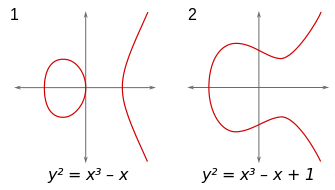
\includegraphics{Figures/ECClines-3.jpg}
    \caption{}
    \label{fig:my_label}
\end{figure}

We will denote the elliptic curve over $K$, as the set $E(K)$ such that
\begin{equation}
    E(K)=\{(x,y) \in K^2 | y^2=x^3+ax+b, a,b \in K\} \cup \{\mathcal{O}\}
\end{equation}


\hspace{10mm} The use of elliptic curves has risen because it provides equivalent security compared to other systems like RSA (Rivest-Shamir-Adleman), but with the use of fewer bits. A typical Elliptic Curve Cryptosystem key size of 256 bits has the same security as an RSA key of 3072 bits. So, on the long run, RSA keys have to get exponentially large to provide equivalent security compared to the fewer bits that the Elliptic Curves Cryptosystem can provide. Another reason for their use is that it becomes an alternative in case that a major weakness is RSA is found. 

\hspace{10mm}  Other reasons for why this cryptosystem has been beneficial is because it is faster than systems like RSA. This is because of the use of smaller keys, which means that less data will be transmitted from server to client. Also, it will take less processing power (CPU) which will again, bring faster responses. \footnote{Thayer, W. (2015, April 04)}



\include{ProblemStatement}
\chapter{Proofs and Demonstrations}

\section{Addition over Elliptic Curves and The Group Law}

\hspace{10mm} To construct a suitable notion of addition of points of elliptic curves, let us consider the curve:
\begin{equation}
    E(\R)=\{(x,y) \in \R^2 | y^2=x^3+ax+b; a,b \in \R\} \cup \{\mathcal{O}\}
\end{equation}

\begin{definition}
Let $E(\R)$ be an elliptic curve over the reals and let $P,Q \in E(\R)$. We define $+$ as follows:
\begin{itemize}
    \item If $P=\mathcal{O}$, then $-P=\mathcal{O}$ and $P+Q=Q$. That is, $\mathcal{O}=-\mathcal{O}$ and $\mathcal{O}+Q=Q$.
    
    \item Let $P=(x,y) \in E(\R)$ then $-P=(x,-y) \in E(\R)$.
    
    \item If $P \neq Q$, then take $l=\overline{PQ}$ to be the line that cuts $E(\R)$ at $P$, $Q$, and another point $R$.Then $P+Q=-R$.
\end{itemize}
\end{definition}

\begin{figure}
    \centering
    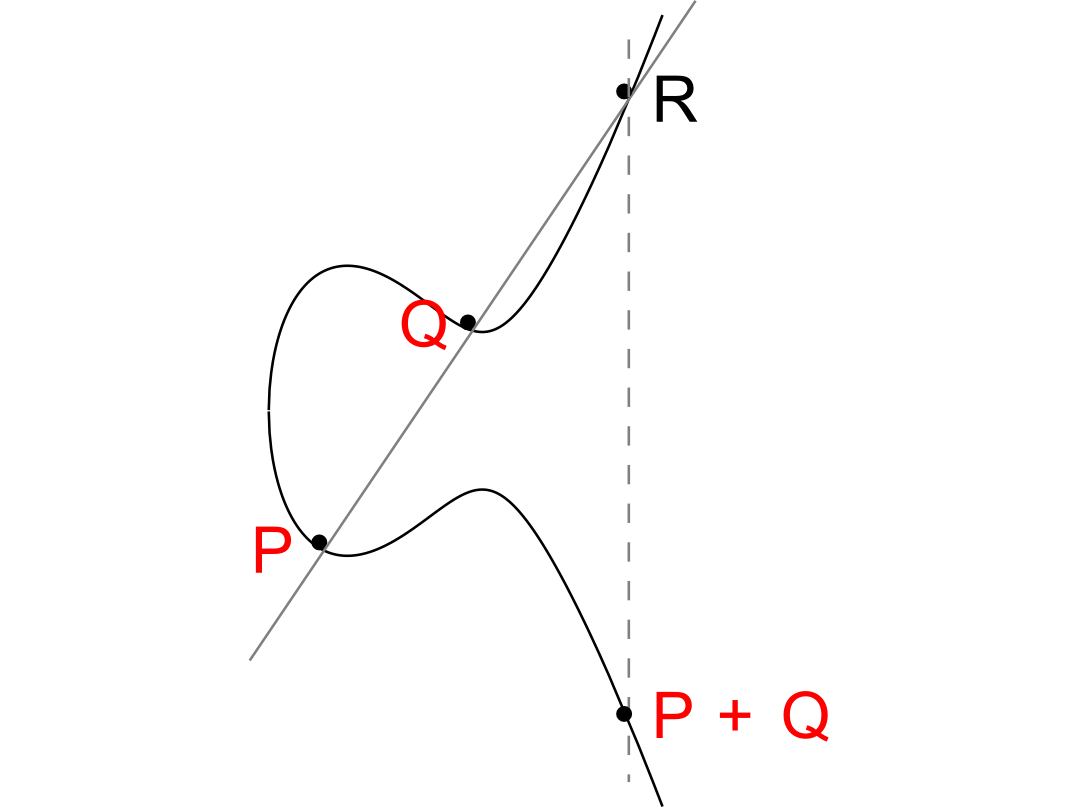
\includegraphics{Figures/EllipticCurveAddition.jpg}
    \caption{Addition of points on an elliptic curve}
    \label{fig:my_label}
\end{figure}

If we let the line $l=\overline{PQ}$ be the plane line $y=\alpha x+\beta$ and $P=(x_1,y_1)$, and $Q=(x_2,y_2)$ be points on $E(\R)$, then we can find the coordinates of $P+Q$ adhering to two cases, the first looks at when $P$ and $Q$ are distinct points, in this case we draw the line that cuts $E(\R)$ at $P$ and $Q$ then we note that $\alpha=\frac{y_2-y_1}{x_2-x_1}$. The latter, concerns itself when $P$ and $Q$ are the same, then it results that the line $y=\alpha x+\beta$ is tangent to the curve, and we consider the derivative of the curve $2y\frac{dy}{dx}=3x^2+a$, and here, $\alpha=\frac{dy}{dx}$, In both cases, $\beta=y_1-\alpha x_1$.

\underline{\keyword{Case 1}} If $P \neq Q$ then $P+Q=(x_3,y_3)$ such that
\begin{equation}
    x_3=(\frac{y_2-y_1}{x_2-x_1})^2-x_1-x_2, y_3=(\frac{y_2-y_1}{x_2-x_1})(x_1-x_1)-y_1
\end{equation}

\underline{\keyword{Case 2}} If $P=Q$ then $P+Q=P+P=(x_3,y_3)$ such that
\begin{equation}
    x_3=(\frac{3x_1^2+a}{2y_1})^2-2x_1, y_3=(\frac{3x_1^2+a}{2y_1})(x_1-x_3)-y_1
\end{equation}

Now that we have found equations for coordinates the point $P+Q$ in $E(\R)$, we can take them to be the coordinates for points on a general elliptic curve $E(K)$.

\hspace{10mm}It can be shown that the elliptic curve $E(K)$ forms an abelian group over $+$, that is for $P,Q,R \in E(K)$:
\begin{itemize}
    \item $P+Q \in E(K)$ (\textit{Closure})
    \item $(P+Q)+R=P+(Q+R)$ (\textit{Associative})
    \item $\exists I \in E(K)$ such that $P+I=I+P=P$ (\textit{Identity Law})
    \item $\exists P^{-1} \in E(K),  \forall P \in E(K)$ such that $P+P^{-1}=P^{-1}+P=I$ (\textit{Inverse Law})
    \item $P+Q=Q+P$ (\textit{Commutative})
\end{itemize}
In fact, it follows by our definition of $+$ over $E(K)$ that commutativity, and the identity and inverse laws are satisfied, where $I=\mathcal{O}$ and $P^{-1}=-P$, it is also rather easy to show closure. Thus, the only law left to prove, is associativity, but the proof for it is beyond the scope of this paper, so we simply accept it as true. In fact, we will go on to prove associativity in a much simpler case in the next section, rather than a general proof. Now that we have gone over addition over elliptic curves and it's properties, we can state the following as a theorem.
\begin{theorem}
    Let $K$ be a field of $characteristic \neq 2,3$ and let $E(K)$ be an elliptic curve, and let $+$ be the addition of points over $E(K)$. Then $(E(K),+)$ forms a group
\end{theorem}

\section{Points of Elliptic Curves Over Finite Fields}

\hspace{10mm}We would like to find elliptitc curves defined over a finite number of points. A natural start, would be to consider the field $\F_q$\footnote{here $\F_q=\Z_q$} where $q=p^r$ for some $r \in \Z$ and where $p$ is prime. For our purposes, it is useful just to consider for now the set $\F_p$ where $p$ is prime.

Consider the elliptic curve:

\begin{equation*}
    E(\F_7)=\{(x,y) \in \F_7^2 | y^2=x^3-x\}\cup\{\mathcal{O}\}
\end{equation*}

where $\F_7=\{\bar{0},\bar{1},\bar{2},\bar{3},\bar{4},\bar{5},\bar{6}\}$. We would like to find the points on the curve $E(\F_7)$. This is achieved simply by finding the points in $\F_7^2$ that satisfy the equation $y^2=x^3-x$:

        \begin{figure}
            \centering
            \begin{tabular}{ |c||c|c|c|c|   }
 \hline
 \multicolumn{5}{|c|}{Points of $y^2=x^3-x$} \\
 \hline
 $x$ & $x^3$ & $x^3-x$ & $y$ & $points$ \\
 \hline
 $\bar{0}$   & $\bar{0}$   & $\bar{0}$ & $\bar{0}$ & $(\bar{0},\bar{0})$ \\
 $\bar{1}$ & $\bar{1}$ & $\bar{0}$ & $\bar{0}$ & $(\bar{1},\bar{0})$ \\
 $\bar{2}$ & $\bar{8}$ & $\bar{6}$ & - & - \\
 $\bar{3}$ & $\bar{2}$ & $\bar{3}$ & - & - \\
 $\bar{4}$ & $\bar{2}$ & $\bar{4}$ & $\bar{2}$,$\bar{5}$ & $(\bar{4}$,$\bar{2})$,$\bar{4}$,$\bar{5})$ \\
 $\bar{5}$ & $\bar{4}$ & $\bar{1}$ & $\bar{1}$,$\bar{6}$ & $(\bar{5}$,$\bar{1})$,$(\bar{5},\bar{6})$ \\
 $\bar{6}$ & $\bar{1}$ & $\bar{0}$ & $\bar{0}$ & $(\bar{6},\bar{0})$ \\
 \hline
\end{tabular}
            \caption{}
            \label{fig:EF7Points}
        \end{figure}

Using \ref{fig:EF7Points} we find that:

\begin{equation*}
    E(\F_7)=\{\mathcal{O},(\bar{0},\bar{0}),(\bar{1},\bar{0}),(\bar{4},\bar{2}),(\bar{4},\bar{5}),(\bar{5},\bar{1}),(\bar{5},\bar{6}),(\bar{6},\bar{0})\}
\end{equation*}

where $|E(\F_7)|=8$. Now that we have found points that satisfy $E(\F_7)$, we would like to establish that this set forms a group over addition\footnote{We would be proving a special case of $E(K)$}. Since it is beyond our scope to prove associativity, we undertake the endeavor of proving it using a cayley table. With this table, we will be able to prove the appropriate group laws.

\begin{theorem}
    Let $+$ be the addition of points on an arbitrary elliptic curve $E(K)$. Then $(E(\F_7),+)$ forms a group.
\end{theorem}
    \begin{proof}
        Since $E(K)$ is closed and commutative under $+$ for any field, $(E(\F_7),+)$ inherits closure and commutativity. Then referring to the cayley table \ref{fig:CayleyTable}
        
        \begin{figure}
            \centering
            \begin{tabular}{l|llllllll}
  + & $\mathcal{O}$ & $(\bar{0},\bar{0})$ & $(\bar{1},\bar{0})$ & $(\bar{4},\bar{2})$ & $(\bar{4},\bar{5})$ & $(\bar{5},\bar{1})$ & $(\bar{5},\bar{6})$ & $(\bar{6},\bar{0})$ \\
\hline
  $\mathcal{O}$ & $\mathcal{O}$ & $(\bar{0},\bar{0})$ & $(\bar{1},\bar{0})$ & $(\bar{4},\bar{2})$ & $(\bar{4},\bar{5})$ & $(\bar{5},\bar{1})$ & $(\bar{5},\bar{6})$ & $(\bar{6},\bar{0})$ \\ 
  $(\bar{0},\bar{0})$ & $(\bar{0},\bar{0})$ & $\mathcal{O}$ & $(\bar{6},\bar{0})$ & $(\bar{5},\bar{1})$ & $(\bar{5},\bar{6})$ & $(\bar{4},\bar{2})$ & $(\bar{4},\bar{5})$ & $(\bar{1},\bar{0})$ \\
  $(\bar{1},\bar{0})$ & $(\bar{1},\bar{0})$ & $(\bar{6},\bar{0})$ & $\mathcal{O}$ & $(\bar{4},\bar{5})$ & $(\bar{4},\bar{2})$ & $(\bar{5},\bar{6})$ & $(\bar{5},\bar{1})$ & $(\bar{0},\bar{0})$ \\
  $(\bar{4},\bar{2})$ & $(\bar{4},\bar{2})$ & $(\bar{5},\bar{1})$ & $(\bar{4},\bar{5})$ & $(\bar{4},\bar{5})$ & $\mathcal{O}$ & $(\bar{6},\bar{0})$ & $(\bar{0},\bar{0})$ & $(\bar{5},\bar{1})$  \\
  $(\bar{4},\bar{5})$ & $(\bar{4},\bar{5})$ & $(\bar{5},\bar{6})$ & $(\bar{4},\bar{2})$ & $\mathcal{O}$ & $(\bar{4},\bar{2})$ & $(\bar{0},\bar{0})$ & $(\bar{6},\bar{0})$ & $(\bar{5},\bar{1})$ \\
  $(\bar{5},\bar{1})$ & $(\bar{5},\bar{1})$ & $(\bar{4},\bar{2})$ & $(\bar{5},\bar{6})$ & $(\bar{6},\bar{0})$ & $(\bar{0},\bar{0})$ & $(\bar{1},\bar{0})$ & $\mathcal{O}$ & $(\bar{5},\bar{6})$ \\
  $(\bar{5},\bar{6})$ & $(\bar{5},\bar{6})$ & $(\bar{4},\bar{5})$ & $(\bar{5},\bar{1})$ & $(\bar{0},\bar{0})$ & $(\bar{6},\bar{0})$ & $\mathcal{O}$ & $(\bar{1},\bar{0})$ & $(\bar{5},\bar{1})$ \\
  $(\bar{6},\bar{0})$ & $(\bar{6},\bar{0})$ & $(\bar{1},\bar{0})$ & $(\bar{0},\bar{0})$ & $(\bar{5},\bar{1})$ & $(\bar{5},\bar{1})$ & $(\bar{5},\bar{6})$ & $(\bar{1},\bar{0})$ & $\mathcal{O}$ \\
\end{tabular}

            \caption{}
            \label{fig:CayleyTable}
        \end{figure}
        
We see from \ref{fig:CayleyTable} that the Inverse and Identity laws are satisfied, furthermore, associativity is satisfied. For example we see that:
        \begin{equation*}
            ((\bar{4},\bar{5})+(\bar{5},\bar{1}))+(\bar{4},\bar{2}) = (\bar{0},\bar{0})+(\bar{4},\bar{2})= (\bar{5},\bar{1})
        \end{equation*}
and
        \begin{equation*}
            (\bar{4},\bar{5})+((\bar{5},\bar{1})+(\bar{4},\bar{2})) = (\bar{4},\bar{5})+(\bar{6},\bar{0}) = (\bar{5},\bar{1})
        \end{equation*}
so 
        \begin{equation*}
            ((\bar{4},\bar{5})+(\bar{5},\bar{1}))+(\bar{4},\bar{2}) = (\bar{4},\bar{5})+((\bar{5},\bar{1})+(\bar{4},\bar{2}))
        \end{equation*}
Therefore we see that $E(\F_7)$ satisfies the group laws, along with commutativity and hence is an abelian group.
    \end{proof}
        \begin{remark}
            In essence $E(\F_7)$ didn't need to inherit closure or commutativity from $E(K)$, as the cayley table \ref{fig:CayleyTable} establishes both properties. We could  have shown closure and commutativity independently; but we would like $E(\F_7)$ to have some dependence on $E(K)$ as to illustrate the group structure of $E(K)$
        \end{remark}
        
\hspace{10mm}We find of all the elements in $E(\F_7)$ that $\mathcal{O}$ is its own inverse\footnote{rote, since $\mathcal{O}$ is the identity element}, the elements $(\bar{0},\bar{0})$, $(\bar{1},\bar{0})$ and $(\bar{6},\bar{0})$ also share this property, they also have the same order. The elements $(\bar{4},\bar{2})$ and $(\bar{4},\bar{5})$ are each others inverse and share the same order, and the same can be said for $(\bar{5},\bar{1})$ and $(\bar{5},\bar{6})$.

        \begin{figure}
            \centering
            \begin{tabular}{l|ll}
        Inverses & Order \\
 \hline
        $\mathcal{O}=-\mathcal{O}$ & $o(\mathcal{O})=1$ \\
        $(\bar{0},\bar{0})=-(\bar{0},\bar{0})$ & $o(\bar{0},\bar{0})=2$ \\
        $(\bar{1},\bar{0})=-(\bar{1},\bar{0})$ & $o(\bar{1},\bar{0})=2$ \\
        $(\bar{4},\bar{2})=-(\bar{4},\bar{5})$ & $o(\bar{4},\bar{2})=3$ \\
        $(\bar{4},\bar{5})=-(\bar{4},\bar{2})$ & $o(\bar{4},\bar{5})=3$ \\
        $(\bar{5},\bar{1})=-(\bar{5},\bar{6})$ & $o(\bar{5},\bar{1})=4$ \\
        $(\bar{5},\bar{6})=-(\bar{5},\bar{1})$ & $o(\bar{5},\bar{1})=4$ \\
        $(\bar{6},\bar{0})=-(\bar{6},\bar{0})$ & $o(\bar{6},\bar{0})=2$ \\
\end{tabular}
            \caption{}
            \label{fig:InverseAndOrder}
        \end{figure}

\hspace{10mm}It is natural to wonder, since the group $E(\F_7)$ has order $8$ whether or not it is isomorphic to some other group like $\Z_8$ which also has order $8$. Since we know that $\Z_8=\{[0],[1],[2],[3],[4],[5],[6],[7]\}$\footnote{To distinguish between the elements of equivalence classes in $\F_7$ and $\Z_8$ we take $\bar{a}$ to be an element of $\F_8$ and $[a]$ an element of $Z_8$}, let $\phi:E(\F_7) \rightarrow \Z_8$ be a isomorphism between $E(\F_7)$ and $\Z_8$. Then for every element $P \in E(\F_7)$, $\phi(P) \in  \Z_8$ and the properties of every $P$ carry over to $\phi(P)$. Hence, $\phi$ takes the group structure and properties of $E(\F_7)$ into $\Z_8$. Now $\Z_8$ is cyclic with respect to $[1]$ (that is $\langle[1]\rangle=\Z_8$), then $[1]$ has order 8. Since $\phi$ is an isomorphism, there must exist some $P \in E(\F_7)$ such that $\phi(P)=[1]$, hence $P$ must have order 8. However referring to \ref{fig:InverseAndOrder}, $E(\F_7)$ has no such element whose order 8. Therefore such a $\phi$ cannot exist, and we see that $E(\F_7)$ is not isomorphic to $\Z_8$.
    \begin{remark}
        It is also sufficient to show that since $E(\F_7)$ has no element of order 8, that it cannot be cyclic with respect to any element, so isomorphism with $\Z_8$ again fails to hold.
    \end{remark}
    

\section{Analog of Massey-Omura}

\hspace{10mm} The Analog of Massey–Omura Cryptosystem was proposed by James Massey and Jim K. Omura in 1982. It is a public key cryptosystem which transmits a message m as points on an elliptic curve E over the field $\F_q$,  where $q=p^r$ for some $r \in \Z$ and $p$, prime. Here, the elliptic curve, as well as its points are public and fixed. The number N of points of E is also known. The protocol for message sending is as follows:

\begin{itemize}
\item The message will be embedded as points on the elliptic curve and will be denoted $P_m$. A prime modulus p will be chosen between both users.
\item Each user (sender A and receiver B) will choose a random integer e such that $1<e<N$ and $(e,N)=1$. Because these e’s will be different for each, we will denote them $e_a$ and $e_b$. This element e will be called encryption key.
\item The users will then calculate their respective decryption keys, which will be in the form d= $\left\{ d \mid e \times d=1 (modN)\right\}$. This is done using the Euclidean Algorithm and will be denoted $d_a$ and $d_b$ respectively.
\item The sender enciphers $P_m$ by computing $e_aP_m$ mod p. This point will be sent to the receiver.
\item The receiver would not be able to retrieve $P_m$ from $e_aP_m$, since he does not know what neither $P_m$ or $e_a$ are. Instead, he will compute $e_be_aP_m$ and will send it to the original sender.

\item The sender will partially decipher the message by computing his decryption key $d_ae_be_aP_m$ and since $d_a \times e_a = 1 (modN)$, this will be $e_bP_m (modN)$ and will be sent to the receiver yet again.

\item The receiver will finish decryption of the message by computing his decryption key $d_be_bP_m (modN)$ which will give $P_m$ which is the original message.\footnote{Koblitz, N. (1994)}

\end{itemize}


\hspace{10mm} Note that someone who might want to intercept the message will only be able to know $e_aP_m, e_bP_M$ and $e_be_aP_m$ and it is not easy to get $P_m$ from those.



\chapter{Open Problems and Future Directions}

\hspace{10mm} This work provided some basic definitions and showed some properties of elliptic curves as a whole. In a future project, types of elliptic curves could be studied as well as explore elliptic curves with characteristic 2 or 3. Additionally, elliptic curves could be studied over the complex and the rationals.

\hspace{10mm} More examples of elliptic curves could be presented as well as all of the calculations done for the one in this work but for each of them. This would show how the formulas work for different forms of elliptic curves. Also, in a future work, an isomorphism could be found with the example elliptic curve provided in this work as well as for others that could be added. 

\hspace{10mm} The elliptic curve discrete logarithm problem (ECDLP) is where the elliptic curve crypstosystem draws its strength. This could be further explained in a future work. Other types of cryptosystems that use elliptic curves such as the analog of Massey Omura could be described in a future project, these may include analog of Diffie–Hellman (ECDH) and analog of ElGamal. 

\chapter{References}
 
 \bibitem{Elliptic}
 [1] Castryck, W. (2013, September 11). Introduction to Elliptic Curve Cryptography. Retrieved from https://www.cosic.esat.kuleuven.be/ecc2013/files/wouter.pdf
 
 \bibitem{Elliptic}
 [2] Brown, E. (2010, December). Elliptic Curve Cryptography. Retrieved from https://www.math.hmc.edu/~ursula/teaching/math189/finalpapers/elaine.pdf
 
 \bibitem{Elliptic}
 [3] Koblitz, N. (1994). A course in number theory and cryptography. Seattle, WA: Springer.
 
 \bibitem{Elliptic}
 [4] Thayer, W. (2015, April 04). Benefits of Elliptic Curve Cryptography. Retrieved from https://casecurity.org/2014/06/10/benefits-of-elliptic-curve-cryptography/
 
 \bibitem{Elliptic}
 [5] Winston, R. (n.d.). Enhancing the Massey-Omura Cryptosystem. Journal of Mathematical Sciences & Mathematics Education, 21-29. Retrieved from http://www.msme.us/2007-1-3.pdf
 
\bibitem{Elliptic}
[6] Koblitz, N. (1987, January). Elliptic Curve Cryptosystems. American Mathematical Society, 203-209. Retrieved from https://www.ams.org/journals/mcom/1987-48-177/S0025-5718-1987-0866109-5/S0025-5718-1987-0866109-5.pdf
%\include{Chapters/Chapter4} 
%\include{Chapters/Chapter5} 

%----------------------------------------------------------------------------------------
%	THESIS CONTENT - APPENDICES
%----------------------------------------------------------------------------------------

\appendix % Cue to tell LaTeX that the following "chapters" are Appendices

% Include the appendices of the thesis as separate files from the Appendices folder
% Uncomment the lines as you write the Appendices

%% Appendix
%==========================================================================
\chapter{}
\label{AppA}

%% Appendix
%==========================================================================
\chapter{TITLE OF APPENDIX B}
\label{AppB}


Appendix B goes here.
%\include{Appendices/AppendixC}

%----------------------------------------------------------------------------------------
%	BIBLIOGRAPHY
%----------------------------------------------------------------------------------------

\printbibliography[heading=bibintoc]

%----------------------------------------------------------------------------------------

\end{document}  
